
\documentclass[dissertation.tex]{subfiles}


%% ODER: format ==         = "\mathrel{==}"
%% ODER: format /=         = "\neq "
%
%
\makeatletter
\@ifundefined{lhs2tex.lhs2tex.sty.read}%
  {\@namedef{lhs2tex.lhs2tex.sty.read}{}%
   \newcommand\SkipToFmtEnd{}%
   \newcommand\EndFmtInput{}%
   \long\def\SkipToFmtEnd#1\EndFmtInput{}%
  }\SkipToFmtEnd

\newcommand\ReadOnlyOnce[1]{\@ifundefined{#1}{\@namedef{#1}{}}\SkipToFmtEnd}
\usepackage{amstext}
\usepackage{amssymb}
\usepackage{stmaryrd}
\DeclareFontFamily{OT1}{cmtex}{}
\DeclareFontShape{OT1}{cmtex}{m}{n}
  {<5><6><7><8>cmtex8
   <9>cmtex9
   <10><10.95><12><14.4><17.28><20.74><24.88>cmtex10}{}
\DeclareFontShape{OT1}{cmtex}{m}{it}
  {<-> ssub * cmtt/m/it}{}
\newcommand{\texfamily}{\fontfamily{cmtex}\selectfont}
\DeclareFontShape{OT1}{cmtt}{bx}{n}
  {<5><6><7><8>cmtt8
   <9>cmbtt9
   <10><10.95><12><14.4><17.28><20.74><24.88>cmbtt10}{}
\DeclareFontShape{OT1}{cmtex}{bx}{n}
  {<-> ssub * cmtt/bx/n}{}
\newcommand{\tex}[1]{\text{\texfamily#1}}	% NEU

\newcommand{\Sp}{\hskip.33334em\relax}


\newcommand{\Conid}[1]{\mathit{#1}}
\newcommand{\Varid}[1]{\mathit{#1}}
\newcommand{\anonymous}{\kern0.06em \vbox{\hrule\@width.5em}}
\newcommand{\plus}{\mathbin{+\!\!\!+}}
\newcommand{\bind}{\mathbin{>\!\!\!>\mkern-6.7mu=}}
\newcommand{\rbind}{\mathbin{=\mkern-6.7mu<\!\!\!<}}% suggested by Neil Mitchell
\newcommand{\sequ}{\mathbin{>\!\!\!>}}
\renewcommand{\leq}{\leqslant}
\renewcommand{\geq}{\geqslant}
\usepackage{polytable}

%mathindent has to be defined
\@ifundefined{mathindent}%
  {\newdimen\mathindent\mathindent\leftmargini}%
  {}%

\def\resethooks{%
  \global\let\SaveRestoreHook\empty
  \global\let\ColumnHook\empty}
\newcommand*{\savecolumns}[1][default]%
  {\g@addto@macro\SaveRestoreHook{\savecolumns[#1]}}
\newcommand*{\restorecolumns}[1][default]%
  {\g@addto@macro\SaveRestoreHook{\restorecolumns[#1]}}
\newcommand*{\aligncolumn}[2]%
  {\g@addto@macro\ColumnHook{\column{#1}{#2}}}

\resethooks

\newcommand{\onelinecommentchars}{\quad-{}- }
\newcommand{\commentbeginchars}{\enskip\{-}
\newcommand{\commentendchars}{-\}\enskip}

\newcommand{\visiblecomments}{%
  \let\onelinecomment=\onelinecommentchars
  \let\commentbegin=\commentbeginchars
  \let\commentend=\commentendchars}

\newcommand{\invisiblecomments}{%
  \let\onelinecomment=\empty
  \let\commentbegin=\empty
  \let\commentend=\empty}

\visiblecomments

\newlength{\blanklineskip}
\setlength{\blanklineskip}{0.66084ex}

\newcommand{\hsindent}[1]{\quad}% default is fixed indentation
\let\hspre\empty
\let\hspost\empty
\newcommand{\NB}{\textbf{NB}}
\newcommand{\Todo}[1]{$\langle$\textbf{To do:}~#1$\rangle$}

\EndFmtInput
\makeatother
%
%
%
%
%
%
% This package provides two environments suitable to take the place
% of hscode, called "plainhscode" and "arrayhscode". 
%
% The plain environment surrounds each code block by vertical space,
% and it uses \abovedisplayskip and \belowdisplayskip to get spacing
% similar to formulas. Note that if these dimensions are changed,
% the spacing around displayed math formulas changes as well.
% All code is indented using \leftskip.
%
% Changed 19.08.2004 to reflect changes in colorcode. Should work with
% CodeGroup.sty.
%
\ReadOnlyOnce{polycode.fmt}%
\makeatletter

\newcommand{\hsnewpar}[1]%
  {{\parskip=0pt\parindent=0pt\par\vskip #1\noindent}}

% can be used, for instance, to redefine the code size, by setting the
% command to \small or something alike
\newcommand{\hscodestyle}{}

% The command \sethscode can be used to switch the code formatting
% behaviour by mapping the hscode environment in the subst directive
% to a new LaTeX environment.

\newcommand{\sethscode}[1]%
  {\expandafter\let\expandafter\hscode\csname #1\endcsname
   \expandafter\let\expandafter\endhscode\csname end#1\endcsname}

% "compatibility" mode restores the non-polycode.fmt layout.

\newenvironment{compathscode}%
  {\par\noindent
   \advance\leftskip\mathindent
   \hscodestyle
   \let\\=\@normalcr
   \let\hspre\(\let\hspost\)%
   \pboxed}%
  {\endpboxed\)%
   \par\noindent
   \ignorespacesafterend}

\newcommand{\compaths}{\sethscode{compathscode}}

% "plain" mode is the proposed default.
% It should now work with \centering.
% This required some changes. The old version
% is still available for reference as oldplainhscode.

\newenvironment{plainhscode}%
  {\hsnewpar\abovedisplayskip
   \advance\leftskip\mathindent
   \hscodestyle
   \let\hspre\(\let\hspost\)%
   \pboxed}%
  {\endpboxed%
   \hsnewpar\belowdisplayskip
   \ignorespacesafterend}

\newenvironment{oldplainhscode}%
  {\hsnewpar\abovedisplayskip
   \advance\leftskip\mathindent
   \hscodestyle
   \let\\=\@normalcr
   \(\pboxed}%
  {\endpboxed\)%
   \hsnewpar\belowdisplayskip
   \ignorespacesafterend}

% Here, we make plainhscode the default environment.

\newcommand{\plainhs}{\sethscode{plainhscode}}
\newcommand{\oldplainhs}{\sethscode{oldplainhscode}}
\plainhs

% The arrayhscode is like plain, but makes use of polytable's
% parray environment which disallows page breaks in code blocks.

\newenvironment{arrayhscode}%
  {\hsnewpar\abovedisplayskip
   \advance\leftskip\mathindent
   \hscodestyle
   \let\\=\@normalcr
   \(\parray}%
  {\endparray\)%
   \hsnewpar\belowdisplayskip
   \ignorespacesafterend}

\newcommand{\arrayhs}{\sethscode{arrayhscode}}

% The mathhscode environment also makes use of polytable's parray 
% environment. It is supposed to be used only inside math mode 
% (I used it to typeset the type rules in my thesis).

\newenvironment{mathhscode}%
  {\parray}{\endparray}

\newcommand{\mathhs}{\sethscode{mathhscode}}

% texths is similar to mathhs, but works in text mode.

\newenvironment{texthscode}%
  {\(\parray}{\endparray\)}

\newcommand{\texths}{\sethscode{texthscode}}

% The framed environment places code in a framed box.

\def\codeframewidth{\arrayrulewidth}
\RequirePackage{calc}

\newenvironment{framedhscode}%
  {\parskip=\abovedisplayskip\par\noindent
   \hscodestyle
   \arrayrulewidth=\codeframewidth
   \tabular{@{}|p{\linewidth-2\arraycolsep-2\arrayrulewidth-2pt}|@{}}%
   \hline\framedhslinecorrect\\{-1.5ex}%
   \let\endoflinesave=\\
   \let\\=\@normalcr
   \(\pboxed}%
  {\endpboxed\)%
   \framedhslinecorrect\endoflinesave{.5ex}\hline
   \endtabular
   \parskip=\belowdisplayskip\par\noindent
   \ignorespacesafterend}

\newcommand{\framedhslinecorrect}[2]%
  {#1[#2]}

\newcommand{\framedhs}{\sethscode{framedhscode}}

% The inlinehscode environment is an experimental environment
% that can be used to typeset displayed code inline.

\newenvironment{inlinehscode}%
  {\(\def\column##1##2{}%
   \let\>\undefined\let\<\undefined\let\\\undefined
   \newcommand\>[1][]{}\newcommand\<[1][]{}\newcommand\\[1][]{}%
   \def\fromto##1##2##3{##3}%
   \def\nextline{}}{\) }%

\newcommand{\inlinehs}{\sethscode{inlinehscode}}

% The joincode environment is a separate environment that
% can be used to surround and thereby connect multiple code
% blocks.

\newenvironment{joincode}%
  {\let\orighscode=\hscode
   \let\origendhscode=\endhscode
   \def\endhscode{\def\hscode{\endgroup\def\@currenvir{hscode}\\}\begingroup}
   %\let\SaveRestoreHook=\empty
   %\let\ColumnHook=\empty
   %\let\resethooks=\empty
   \orighscode\def\hscode{\endgroup\def\@currenvir{hscode}}}%
  {\origendhscode
   \global\let\hscode=\orighscode
   \global\let\endhscode=\origendhscode}%

\makeatother
\EndFmtInput
%
%
%
% First, let's redefine the forall, and the dot.
%
%
% This is made in such a way that after a forall, the next
% dot will be printed as a period, otherwise the formatting
% of `comp_` is used. By redefining `comp_`, as suitable
% composition operator can be chosen. Similarly, period_
% is used for the period.
%
\ReadOnlyOnce{forall.fmt}%
\makeatletter

% The HaskellResetHook is a list to which things can
% be added that reset the Haskell state to the beginning.
% This is to recover from states where the hacked intelligence
% is not sufficient.

\let\HaskellResetHook\empty
\newcommand*{\AtHaskellReset}[1]{%
  \g@addto@macro\HaskellResetHook{#1}}
\newcommand*{\HaskellReset}{\HaskellResetHook}

\global\let\hsforallread\empty

\newcommand\hsforall{\global\let\hsdot=\hsperiodonce}
\newcommand*\hsperiodonce[2]{#2\global\let\hsdot=\hscompose}
\newcommand*\hscompose[2]{#1}

\AtHaskellReset{\global\let\hsdot=\hscompose}

% In the beginning, we should reset Haskell once.
\HaskellReset

\makeatother
\EndFmtInput
%




\newmuskip\codemuskip
\codemuskip=4.0mu plus 2.0mu minus 2.0mu\relax
\providecommand\codeskip{\mskip\codemuskip}%
\let\codefont\textsf
\providecommand\sub[1]{\ensuremath{_{\text{#1}}}}
\providecommand\keyw[1]{{\codefont{\textbf{#1}}}}
\providecommand\id[1]{\Varid{#1}}
\providecommand\idsym[1]{\mathbin{\id{#1}}}
\providecommand{\vertrule}[1][1.0ex]{\rule[-0.0ex]{.45pt}{#1}}
\renewcommand\Varid[1]{\codefont{#1}}
\let\Conid\Varid




\begin{document}


\long\def\ignore#1{}
\ignore{
\begin{hscode}\SaveRestoreHook
\column{B}{@{}>{\hspre}l<{\hspost}@{}}%
\column{E}{@{}>{\hspre}l<{\hspost}@{}}%
\>[B]{}\mbox{\enskip\{-\# LANGUAGE KindSignatures, GADTs, LambdaCase, RankNTypes, TypeOperators, OverlappingInstances, DataKinds, FlexibleInstances, FlexibleContexts, MultiParamTypeClasses, TypeFamilies, PolyKinds  \#-\}\enskip}{}\<[E]%
\\
\>[B]{}\mathbf{module}\codeskip \Conid{Background}\codeskip \mathbf{where}{}\<[E]%
\\
\>[B]{}\mathbf{import}\codeskip \Conid{Prelude}\codeskip \Varid{hiding}\codeskip (\Varid{or}){}\<[E]%
\\
\>[B]{}\mathbf{import}\codeskip \Conid{\Conid{Data}.Kind}\codeskip (\Conid{Type}){}\<[E]%
\ColumnHook
\end{hscode}\resethooks
}

\chapter{Background}\label{chap:background}

\section{Dataflow Programming}
Dataflow programming is a paradigm that models applications as a directed graph.
The nodes of the graph have inputs and outputs and are pure functions, therefore have no side effects.
It is possible for a node to be a: source; sink; or processing node.
A source is a read-only storage: it can be used to feed inputs into processes.
A sink is a write-only storage: it can be used to store the outputs of processes.
Processes will read from either a source or the output of another process,
and then produce a result which is either passed to another process or saved in a sink.
Edges connect these nodes together, and define the flow of information.


\paragraph{Example - Data Pipelines}
A common use of dataflow programming is in pipelines that process data.
This paradigm is particularly helpful as it helps the developer to focus on each specific transformation on the data as a single component.
Avoiding the need for long and laborious scripts that could be hard to maintain.
One example of a data pipeline tool that makes use of dataflow programming is Luigi~\cite{spotify_luigi}.
An example dataflow graph produced by the tool is shown in Figure~\ref{fig:luigi-example}

\begin{figure}[ht]
  \centering
  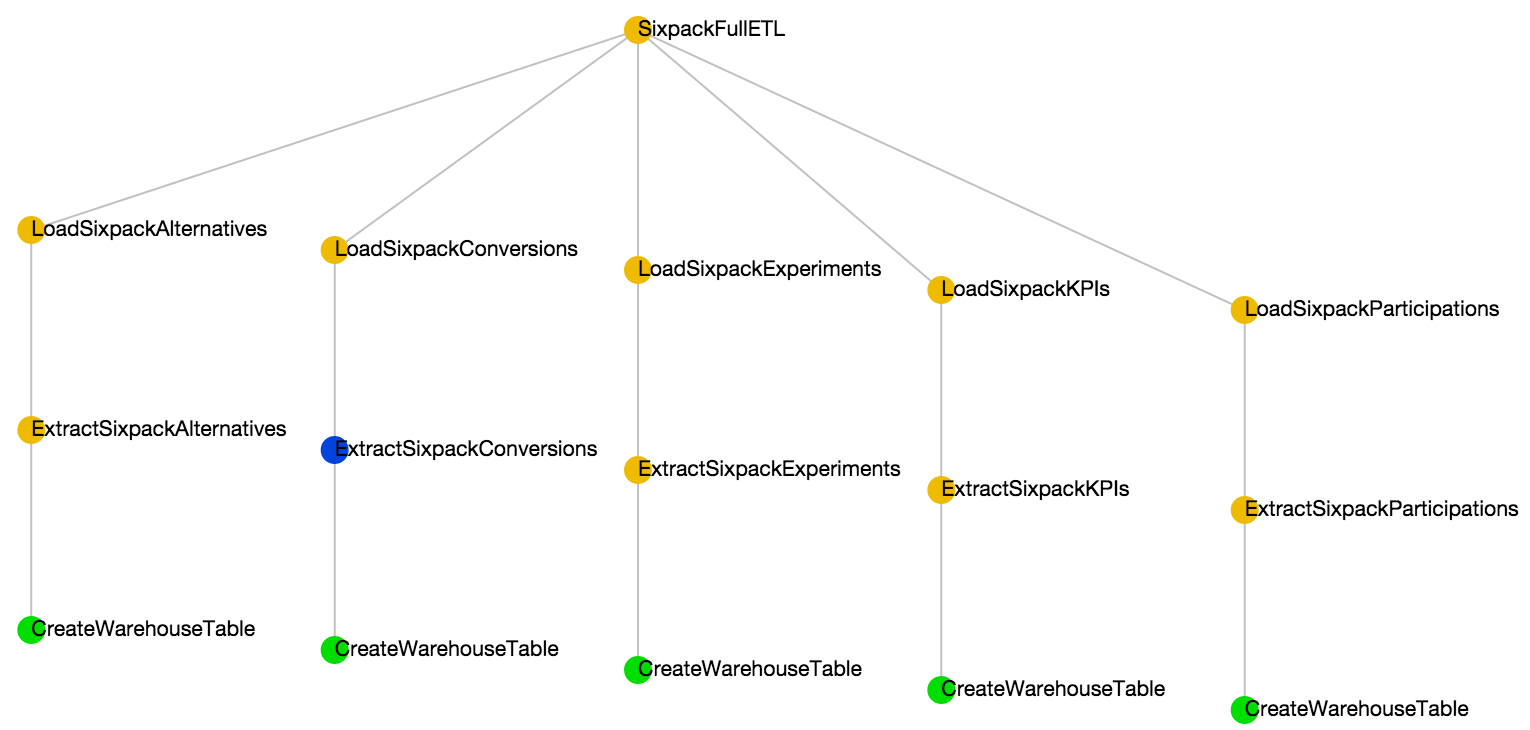
\includegraphics[scale=0.4]{diagrams/luigi-example.png}
  \caption{Luigi dependency graph~\cite{hu_2015}}
  \label{fig:luigi-example}
\end{figure}



\paragraph{Example - Quartz Composer}
Apple developed a tool included in XCode, named Quartz Composer, which is a node-based visual programming language~\cite{quartz}.
As seen in Figure~\ref{fig:quartz-composer}, it uses a visual approach to programming connecting nodes with edges.
This allows for quick development of programs that process and render graphical data, without the user having to write a single line of code.
This means that even non-programmers are able to use the tool.

\begin{figure}[ht]
  \centering
  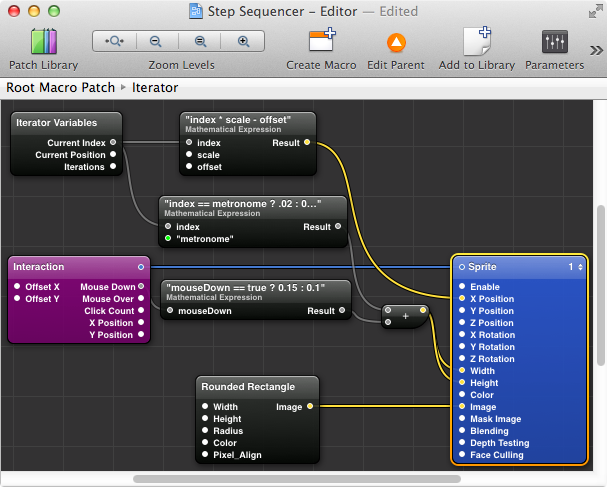
\includegraphics[scale=0.3]{diagrams/quartz_composer.png}
  \caption{Quartz composer~\cite{costello_2012}}
  \label{fig:quartz-composer}
\end{figure}


\paragraph{Example - Spreadsheets}
A widely used example of dataflow programming is in spreadsheets.
A cell in a spreadsheet can be thought of as a single node.
It is possible to specify dependencies to other cells through the use of formulas.
Whenever a cell is updated it sends its new value to those who depend on it, and so on.
Work has also done to visualise spreadsheets using dataflow diagrams, to help debug ones that are complex~\cite{hermans2011breviz}.


\subsection{The Benefits}
\paragraph{Visual}
The dataflow paradigm uses graphs, which make programming visual.
It allows the end-user programmer to see how data passes through the program, much easier than in an imperative approach.
In many cases, dataflow programming languages use drag and drop blocks with a graphical user interface to build programs.
For example, Tableau Prep~\cite{tableauPrep}, that makes programming more accessible to users who do not have programming skills.

\paragraph{Implicit Parallelism}
Moore's law states that the number of transistors on a computer chip doubles every two years~\cite{4785860}.
This meant that the chips' processing speeds also increased in alignment with Moore's law.
However, in recent years this is becoming harder for chip manufacturers to achieve~\cite{bentley_2020}.
Therefore, chip manufactures have had to turn to other approaches to increase the speed of new chips, such as multiple cores.
It is this approach the dataflow programming can effectively make use of.
Since each node in a dataflow is a pure function, it is possible to parallelise implicitly.
No node can interact with another node, therefore there are no data dependencies outside of those encoded in the dataflow.
Thus eliminating the ability for a deadlock to occur.

\subsection{Dataflow Diagrams}
Dataflow programs are typically viewed as a graph.
An example dataflow graph along with its corresponding imperative approach, can be found in Figure~\ref{fig:dataflow-example}.
The nodes $100$, $X$, and $Y$ are sources as they are only read from. $C$ is a sink as it is wrote to.
The remaining nodes are all processes, as they have some number of inputs and compute a result.

\begin{figure}[ht]
  \centering
  \begin{subfigure}{0.3\textwidth}
    \centering
    \begin{equation*}
      \begin{aligned}
      A &:= 100 \times X \\
      B &:= X + Y \\
      C &:= A - B \\
      \end{aligned}
    \end{equation*}
    \caption{}
    \label{subfig:dataflow-example-equations}
  \end{subfigure}
  \begin{subfigure}{0.3\textwidth}
    \centering
    \begin{tikzpicture}[node distance={15mm}, main/.style = {draw, thick}]
\node (100) {$100$};
\node (X)   [right of=100] {$X$};
\node (Y)    [right of=X] {$Y$};
\node[main] (plus) [below right of=X, below left of=Y] {$+$};
\node[main] (mul)  [below right of=100, below left of=X] {$\times$};
\node[main] (sub)  [below right of=mul, below left of=plus] {$-$};
\node (C)    [below of=sub] {$C$};

\draw[->, >=stealth] (100) -- (mul);
\draw[->, >=stealth] (X) -- (mul);
\draw[->, >=stealth] (X) -- (plus);
\draw[->, >=stealth] (Y) -- (plus);
\draw[->, >=stealth] (mul) -- (sub);
\draw[->, >=stealth] (plus) -- (sub);
\draw[->, >=stealth] (sub) -- (C);

\end{tikzpicture}

    \caption{}
    \label{subfig:dataflow-example-diagram}
  \end{subfigure}
  \caption{An example dataflow and its imperative approach.}
    \label{fig:dataflow-example}
\end{figure}

In this diagram is possible to see how implicit parallelisation is possible.
Both $A$ and $B$ can be calculated simultaneously, with $C$ able to be evaluated after they are complete.


\subsection{\acfp{KPN}}
A method introduced by Gilles Kahn, \acfp{KPN} realised the concept of dataflow networks
through the use of threads and unbounded \ac{FIFO} queues~\cite{DBLP:conf/ifip/Kahn74}.
The \ac{FIFO} queue is one where the items are output in the same order that they are added.
A node in the dataflow becomes a thread in the process network.
Each \ac{FIFO} queue represents the edges connecting the nodes in a graph.
The threads are then able to communicate through \ac{FIFO} queues.
The node can have multiple input queues and is able to read any number of values from them.
It will then compute a result and add it to an output queue.
Kahn imposed a restriction on a process in a \acp{KPN} that the thread is suspended if it attempts to fetch a value from an empty queue.
The thread is not allowed to test for the presence of data in a queue.

\begin{figure}[ht]
  \centering
  \usetikzlibrary{decorations.markings}
\tikzset{-dot-/.style={decoration={
  markings,
  mark=at position #1 with {\fill circle (2pt);}},postaction={decorate}}}

\begin{subfigure}{0.3\textwidth}
\centering
\begin{tikzpicture}[node distance={30mm}, main/.style = {draw, circle, thick}, fired/.style = {draw, circle, thick, fill=black, text=white}]
\node[fired] (1) {$1$};
\node[main] (2) [right of=1] {$2$};
\draw[->, >=stealth, -dot-=0.5] (1) -- (2);
\end{tikzpicture}
\caption{}
\end{subfigure}

\begin{subfigure}{0.3\textwidth}
\centering
\begin{tikzpicture}[node distance={30mm}, main/.style = {draw, circle, thick}, fired/.style = {draw, circle, thick, fill=black, text=white}]
\node[fired] (1) {$1$};
\node[main] (2) [right of=1] {$2$};
\draw[->, >=stealth, -dot-=0.55, -dot-=0.45] (1) -- (2);
\end{tikzpicture}
\caption{}
\end{subfigure}

\begin{subfigure}{0.3\textwidth}
\centering
\begin{tikzpicture}[node distance={30mm}, main/.style = {draw, circle, thick}, fired/.style = {draw, circle, thick, fill=black, text=white}]
\node[main] (1) {$1$};
\node[fired] (2) [right of=1] {$2$};
\draw[->, >=stealth, -dot-=0.5] (1) -- (2);
\end{tikzpicture}
\caption{}
\end{subfigure}

\begin{subfigure}{0.3\textwidth}
\centering
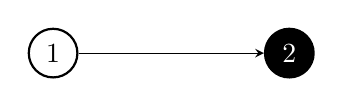
\begin{tikzpicture}[node distance={30mm}, main/.style = {draw, circle, thick}, fired/.style = {draw, circle, thick, fill=black, text=white}]
\node[main] (1) {$1$};
\node[fired] (2) [right of=1] {$2$};
\draw[->, >=stealth] (1) -- (2);
\end{tikzpicture}
\caption{}
\end{subfigure}

% \begin{subfigure}{0.34\textwidth}
% \centering
% \begin{tikzpicture}[node distance={30mm}, main/.style = {draw, circle, thick}, fired/.style = {draw, circle, thick, fill=black, text=white}]
% \node[fired] (1) {$1$};
% \node[main] (2) [right of=1] {$2$};
% \draw[->, >=stealth, -dot-=0.5, -dot-=0.1] (1) -- (2);
% \end{tikzpicture}
% \caption{}
% \end{subfigure}

  \caption{A sequence of node firings in a \ac{KPN}}
  \label{fig:kpn-firing}
\end{figure}

Parks described a variant of \acp{KPN}, called \acp{DPN}~\cite{381846}.
They recognise that if functions have no side effects then they have no values to be shared between each firing.
Therefore, a pool of threads can be used with a central scheduler instead.



\section{\acfp{DSL}}
A \ac{DSL} is a programming language that has a specialised domain or use-case.
This differs from a \ac{GPL}, which can be applied across a larger set of domains, and are generally turing complete.
HTML is an example of a \ac{DSL}: it is good for describing the appearance of websites, however,
it cannot be used for more generic purposes, such as adding two numbers together.

\paragraph{Approaches to Implementation}
DSLs are typically split into two categories: standalone and embedded.
Standalone DSLs require their own compiler and typically their own syntax; HTML would be an example of a standalone \ac{DSL}.
\acp{EDSL} use an existing language as a host, therefore they use the syntax and compiler from the host.
This means that they are easier to maintain and often quicker to develop than standalone \acp{DSL}.
An \ac{EDSL}, can be implemented using two differing techniques: deep and shallow embeddings.



\subsection{Deep Embeddings}
A deep embedding is when the terms of the \ac{DSL} will construct an \ac{AST} as a host language datatype.
Semantics can then be provided later on with evaluation functions.
Consider the example of a minimal non-deterministic parser combinator library~\cite{wuYoda}.


\begin{hscode}\SaveRestoreHook
\column{B}{@{}>{\hspre}l<{\hspost}@{}}%
\column{3}{@{}>{\hspre}l<{\hspost}@{}}%
\column{14}{@{}>{\hspre}l<{\hspost}@{}}%
\column{30}{@{}>{\hspre}l<{\hspost}@{}}%
\column{33}{@{}>{\hspre}l<{\hspost}@{}}%
\column{E}{@{}>{\hspre}l<{\hspost}@{}}%
\>[B]{}\mathbf{data}\codeskip \Conid{Parser}_{\Varid{d}}\codeskip (\Varid{a}\mathbin{::}\Conid{Type})\codeskip \mathbf{where}{}\<[E]%
\\
\>[B]{}\hsindent{3}{}\<[3]%
\>[3]{}\Conid{Satisfy}_{\Varid{d}}{}\<[14]%
\>[14]{}\mathbin{::}(\Conid{Char}\to \Conid{Bool}){}\<[33]%
\>[33]{}\to \Conid{Parser}_{\Varid{d}}\codeskip \Conid{Char}{}\<[E]%
\\
\>[B]{}\hsindent{3}{}\<[3]%
\>[3]{}\Conid{Or}_{\Varid{d}}{}\<[14]%
\>[14]{}\mathbin{::}\Conid{Parser}_{\Varid{d}}\codeskip \Varid{a}{}\<[30]%
\>[30]{}\to \Conid{Parser}_{\Varid{d}}\codeskip \Varid{a}\to \Conid{Parser}_{\Varid{d}}\codeskip \Varid{a}{}\<[E]%
\ColumnHook
\end{hscode}\resethooks

\noindent
This can be used to build a parser that can parse the characters \ensuremath{\text{\ttfamily{\textquotesingle}a\textquotesingle}} or \ensuremath{\text{\ttfamily{\textquotesingle}b\textquotesingle}}.

\begin{hscode}\SaveRestoreHook
\column{B}{@{}>{\hspre}l<{\hspost}@{}}%
\column{E}{@{}>{\hspre}l<{\hspost}@{}}%
\>[B]{}\Varid{aorb}_{\Varid{d}}\mathbin{::}\Conid{Parser}_{\Varid{d}}\codeskip \Conid{Char}{}\<[E]%
\\
\>[B]{}\Varid{aorb}_{\Varid{d}}\mathrel{=}\Conid{Satisfy}_{\Varid{d}}\codeskip (\equiv \text{\ttfamily{\textquotesingle}a\textquotesingle})\mathbin{\text{\`{}}\Conid{Or}_{\Varid{d}}\text{\`{}}}\Conid{Satisfy}_{\Varid{d}}\codeskip (\equiv \text{\ttfamily{\textquotesingle}b\textquotesingle}){}\<[E]%
\ColumnHook
\end{hscode}\resethooks

\noindent
However, this parser does not have any semantics, therefore this needs to be provided by the evaluation function \ensuremath{\Varid{parse}}.

\begin{hscode}\SaveRestoreHook
\column{B}{@{}>{\hspre}l<{\hspost}@{}}%
\column{3}{@{}>{\hspre}l<{\hspost}@{}}%
\column{12}{@{}>{\hspre}l<{\hspost}@{}}%
\column{24}{@{}>{\hspre}l<{\hspost}@{}}%
\column{E}{@{}>{\hspre}l<{\hspost}@{}}%
\>[B]{}\Varid{parse}_{\Varid{d}}\mathbin{::}\Conid{Parser}_{\Varid{d}}\codeskip \Varid{a}\to \Conid{String}\to [\mskip1.5mu (\Varid{a},\Conid{String})\mskip1.5mu]{}\<[E]%
\\
\>[B]{}\Varid{parse}_{\Varid{d}}\codeskip (\Conid{Satisfy}_{\Varid{d}}\codeskip \Varid{p}){}\<[24]%
\>[24]{}\mathrel{=}\lambda \mathbf{case}{}\<[E]%
\\
\>[B]{}\hsindent{3}{}\<[3]%
\>[3]{}[\mskip1.5mu \mskip1.5mu]{}\<[12]%
\>[12]{}\to [\mskip1.5mu \mskip1.5mu]{}\<[E]%
\\
\>[B]{}\hsindent{3}{}\<[3]%
\>[3]{}(\Varid{t}\mathbin{:}\Varid{ts'}){}\<[12]%
\>[12]{}\to [\mskip1.5mu (\Varid{t},\Varid{ts'})\mid \Varid{p}\codeskip \Varid{t}\mskip1.5mu]{}\<[E]%
\\
\>[B]{}\Varid{parse}_{\Varid{d}}\codeskip (\Conid{Or}_{\Varid{d}}\codeskip \Varid{px}\codeskip \Varid{py}){}\<[24]%
\>[24]{}\mathrel{=}\lambda \Varid{ts}\to \Varid{parse}_{\Varid{d}}\codeskip \Varid{px}\codeskip \Varid{ts}\plus \Varid{parse}_{\Varid{d}}\codeskip \Varid{py}\codeskip \Varid{ts}{}\<[E]%
\ColumnHook
\end{hscode}\resethooks

\noindent
The program can then be evaluated by the \ensuremath{\Varid{parse}_{\Varid{d}}} function.
For example, \ensuremath{\Varid{parse}_{\Varid{d}}\codeskip \Varid{aorb}_{\Varid{d}}\codeskip \text{\ttfamily \char34 a\char34}} evaluates to \ensuremath{[\mskip1.5mu (\text{\ttfamily{\textquotesingle}a\textquotesingle},\text{\ttfamily \char34 \char34})\mskip1.5mu]}, and \ensuremath{\Varid{parse}_{\Varid{d}}\codeskip \Varid{aorb}_{\Varid{d}}\codeskip \text{\ttfamily \char34 c\char34}} evaluates to \ensuremath{[\mskip1.5mu \mskip1.5mu]}.

A key benefit for deep embeddings is that the structure can be inspected, and then modified to optimise the user code: Parsley~\cite{parsley} makes use of such techniques to create optimised parsers.
Another benefit, is that you can provide multiple interpretations, by specifying different evaluation functions.
However, they also have drawbacks - it can be laborious to add a new constructor to the language.
Since it requires that all functions that use the deep embedding be modified to add a case for the new constructor \cite{SVENNINGSSON2015143}.

\subsection{Shallow Embeddings}
In contrast, a shallow approach is when the terms of the \ac{DSL} are defined as first class components of the language.
For example, a function in Haskell.
Components can then be composed together and evaluated to provide the semantics of the language.
Again a simple parser example can be considered.


\begin{hscode}\SaveRestoreHook
\column{B}{@{}>{\hspre}l<{\hspost}@{}}%
\column{3}{@{}>{\hspre}l<{\hspost}@{}}%
\column{12}{@{}>{\hspre}l<{\hspost}@{}}%
\column{E}{@{}>{\hspre}l<{\hspost}@{}}%
\>[B]{}\mathbf{newtype}\codeskip \Conid{Parser}_{\Varid{s}}\codeskip \Varid{a}\mathrel{=}\Conid{Parser}_{\Varid{s}}\codeskip \{\mskip1.5mu \Varid{parse}_{\Varid{s}}\mathbin{::}\Conid{String}\to [\mskip1.5mu (\Varid{a},\Conid{String})\mskip1.5mu]\mskip1.5mu\}{}\<[E]%
\\[\blanklineskip]%
\>[B]{}\Varid{or}_{\Varid{s}}\mathbin{::}\Conid{Parser}_{\Varid{s}}\codeskip \Varid{a}\to \Conid{Parser}_{\Varid{s}}\codeskip \Varid{a}\to \Conid{Parser}_{\Varid{s}}\codeskip \Varid{a}{}\<[E]%
\\
\>[B]{}\Varid{or}_{\Varid{s}}\codeskip (\Conid{Parser}_{\Varid{s}}\codeskip \Varid{px})\codeskip (\Conid{Parser}_{\Varid{s}}\codeskip \Varid{py})\mathrel{=}\Conid{Parser}_{\Varid{s}}\codeskip (\lambda \Varid{ts}\to \Varid{px}\codeskip \Varid{ts}\plus \Varid{py}\codeskip \Varid{ts}){}\<[E]%
\\[\blanklineskip]%
\>[B]{}\Varid{satisfy}_{\Varid{s}}\mathbin{::}(\Conid{Char}\to \Conid{Bool})\to \Conid{Parser}_{\Varid{s}}\codeskip \Conid{Char}{}\<[E]%
\\
\>[B]{}\Varid{satisfy}_{\Varid{s}}\codeskip \Varid{p}\mathrel{=}\Conid{Parser}_{\Varid{s}}\codeskip (\lambda \mathbf{case}{}\<[E]%
\\
\>[B]{}\hsindent{3}{}\<[3]%
\>[3]{}[\mskip1.5mu \mskip1.5mu]{}\<[12]%
\>[12]{}\to [\mskip1.5mu \mskip1.5mu]{}\<[E]%
\\
\>[B]{}\hsindent{3}{}\<[3]%
\>[3]{}(\Varid{t}\mathbin{:}\Varid{ts'}){}\<[12]%
\>[12]{}\to [\mskip1.5mu (\Varid{t},\Varid{ts'})\mid \Varid{p}\codeskip \Varid{t}\mskip1.5mu]){}\<[E]%
\ColumnHook
\end{hscode}\resethooks

\noindent
The same \ensuremath{\Varid{aorb}_{\Varid{s}}} parser can be constructed from these functions, avoiding the need for an intermediate \ac{AST}.

\begin{hscode}\SaveRestoreHook
\column{B}{@{}>{\hspre}l<{\hspost}@{}}%
\column{E}{@{}>{\hspre}l<{\hspost}@{}}%
\>[B]{}\Varid{aorb}_{\Varid{s}}\mathbin{::}\Conid{Parser}_{\Varid{s}}\codeskip \Conid{Char}{}\<[E]%
\\
\>[B]{}\Varid{aorb}_{\Varid{s}}\mathrel{=}\Varid{satisfy}_{\Varid{s}}\codeskip (\equiv \text{\ttfamily{\textquotesingle}a\textquotesingle})\mathbin{\text{\`{}}\Varid{or}_{\Varid{s}}\text{\`{}}}\Varid{satisfy}_{\Varid{s}}\codeskip (\equiv \text{\ttfamily{\textquotesingle}b\textquotesingle}){}\<[E]%
\ColumnHook
\end{hscode}\resethooks


Using a shallow implementation has the benefit of being able add new `constructors' to a \ac{DSL}, without having to modify any other functions.
Since each `constructor', produces the desired result directly.
However, this causes one of the main disadvantages of a shallow embedding - the structure cannot be inspected.
This means that optimisations cannot be made to the structure before evaluating it.


\section{Higher Order Functors}\label{sec:higher-order-functors}

It is possible to capture the shape of an abstract datatype as a \ensuremath{\Conid{Functor}}.
The use of a \ensuremath{\Conid{Functor}} allows for the specification of where a datatype recurses.
Consider an example on a small expression language:

\begin{hscode}\SaveRestoreHook
\column{B}{@{}>{\hspre}l<{\hspost}@{}}%
\column{12}{@{}>{\hspre}c<{\hspost}@{}}%
\column{12E}{@{}l@{}}%
\column{15}{@{}>{\hspre}l<{\hspost}@{}}%
\column{20}{@{}>{\hspre}l<{\hspost}@{}}%
\column{E}{@{}>{\hspre}l<{\hspost}@{}}%
\>[B]{}\mathbf{data}\codeskip \Conid{Expr}{}\<[12]%
\>[12]{}\mathrel{=}{}\<[12E]%
\>[15]{}\Conid{Add}\codeskip {}\<[20]%
\>[20]{}\Conid{Expr}\codeskip \Conid{Expr}{}\<[E]%
\\
\>[12]{}\mid {}\<[12E]%
\>[15]{}\Conid{Val}\codeskip {}\<[20]%
\>[20]{}\Conid{Int}{}\<[E]%
\ColumnHook
\end{hscode}\resethooks

The recursion within the \ensuremath{\Conid{Expr}} datatype can be removed to form \ensuremath{\Conid{ExprF}}.
The recursive steps can then be specified in the \ensuremath{\Conid{Functor}} instance.

\begin{hscode}\SaveRestoreHook
\column{B}{@{}>{\hspre}l<{\hspost}@{}}%
\column{3}{@{}>{\hspre}l<{\hspost}@{}}%
\column{15}{@{}>{\hspre}c<{\hspost}@{}}%
\column{15E}{@{}l@{}}%
\column{18}{@{}>{\hspre}l<{\hspost}@{}}%
\column{22}{@{}>{\hspre}l<{\hspost}@{}}%
\column{24}{@{}>{\hspre}l<{\hspost}@{}}%
\column{30}{@{}>{\hspre}l<{\hspost}@{}}%
\column{E}{@{}>{\hspre}l<{\hspost}@{}}%
\>[B]{}\mathbf{data}\codeskip \Conid{ExprF}\codeskip \Varid{f}{}\<[15]%
\>[15]{}\mathrel{=}{}\<[15E]%
\>[18]{}\Conid{AddF}\codeskip {}\<[24]%
\>[24]{}\Varid{f}\codeskip \Varid{f}{}\<[E]%
\\
\>[15]{}\mid {}\<[15E]%
\>[18]{}\Conid{ValF}\codeskip {}\<[24]%
\>[24]{}\Conid{Int}{}\<[E]%
\\[\blanklineskip]%
\>[B]{}\mathbf{instance}\codeskip \Conid{Functor}\codeskip \Conid{ExprF}\codeskip \mathbf{where}{}\<[E]%
\\
\>[B]{}\hsindent{3}{}\<[3]%
\>[3]{}\Varid{fmap}\codeskip \Varid{f}\codeskip (\Conid{AddF}\codeskip \Varid{x}\codeskip \Varid{y}){}\<[22]%
\>[22]{}\mathrel{=}\Conid{AddF}\codeskip {}\<[30]%
\>[30]{}(\Varid{f}\codeskip \Varid{x})\codeskip (\Varid{f}\codeskip \Varid{y}){}\<[E]%
\\
\>[B]{}\hsindent{3}{}\<[3]%
\>[3]{}\Varid{fmap}\codeskip \Varid{f}\codeskip (\Conid{ValF}\codeskip \Varid{x}){}\<[22]%
\>[22]{}\mathrel{=}\Conid{ValF}\codeskip {}\<[30]%
\>[30]{}\Varid{x}{}\<[E]%
\ColumnHook
\end{hscode}\resethooks

To regain a datatype that is isomorphic to the original datatype, the recursive knot need to be tied.
This can be done with \ensuremath{\Conid{Fix}}, to get the fixed point of \ensuremath{\Conid{ExprF}}:

\begin{hscode}\SaveRestoreHook
\column{B}{@{}>{\hspre}l<{\hspost}@{}}%
\column{13}{@{}>{\hspre}l<{\hspost}@{}}%
\column{E}{@{}>{\hspre}l<{\hspost}@{}}%
\>[B]{}\mathbf{data}\codeskip \Conid{Fix}\codeskip \Varid{f}{}\<[13]%
\>[13]{}\mathrel{=}\Conid{In}\codeskip (\Varid{f}\codeskip (\Conid{Fix}\codeskip \Varid{f})){}\<[E]%
\\
\>[B]{}\mathbf{type}\codeskip \Conid{Expr'}{}\<[13]%
\>[13]{}\mathrel{=}\Conid{Fix}\codeskip \Conid{ExprF}{}\<[E]%
\ColumnHook
\end{hscode}\resethooks

There is, however, one problem: a \ensuremath{\Conid{Functor}} expressing the a parser language is required to be typed.
Parsers require the type of the tokens being parsed.
For example, a parser reading tokens that make up an expression could have the type \ensuremath{\Conid{Parser}\codeskip \Conid{Expr}}.
A \ensuremath{\Conid{Functor}} does not retain this type information needed in a parser.

\paragraph{IFunctors}
Instead a type class called \ensuremath{\Conid{IFunctor}} --- also known as \ensuremath{\Conid{HFunctor}} --- can be used, which is able to maintain the type indicies~\cite{mcbride2011functional}.
This makes use of \ensuremath{\leadsto}, which represents a natural transformation from \ensuremath{\Varid{f}} to \ensuremath{\Varid{g}}.
\ensuremath{\Conid{IFunctor}} can be thought of as a functor transformer: it is able to change the structure of a functor, whilst preserving the values inside it~\cite{lane1998categories}.
Whereas a functor changes the values inside a structure.


\begin{hscode}\SaveRestoreHook
\column{B}{@{}>{\hspre}l<{\hspost}@{}}%
\column{3}{@{}>{\hspre}l<{\hspost}@{}}%
\column{E}{@{}>{\hspre}l<{\hspost}@{}}%
\>[B]{}\mathbf{type}\codeskip (\leadsto)\codeskip \Varid{f}\codeskip \Varid{g}\mathrel{=}\forall \Varid{a}\hsforall \hsdot{\cdot }{.}\Varid{f}\codeskip \Varid{a}\to \Varid{g}\codeskip \Varid{a}{}\<[E]%
\\
\>[B]{}\mathbf{class}\codeskip \Conid{IFunctor}\codeskip \Varid{iF}\codeskip \mathbf{where}{}\<[E]%
\\
\>[B]{}\hsindent{3}{}\<[3]%
\>[3]{}\Varid{imap}\mathbin{::}(\Varid{f}\leadsto\Varid{g})\to \Varid{iF}\codeskip \Varid{f}\leadsto\Varid{iF}\codeskip \Varid{g}{}\<[E]%
\ColumnHook
\end{hscode}\resethooks

\noindent
The shape of \ensuremath{\Conid{Parser}} can be seen in \ensuremath{\Conid{ParserF}} where the \ensuremath{\Varid{f}} marks the recursive spots.
The type \ensuremath{\Varid{f}} represents the type of the children of that node.
In most cases this will be itself.

\begin{hscode}\SaveRestoreHook
\column{B}{@{}>{\hspre}l<{\hspost}@{}}%
\column{3}{@{}>{\hspre}l<{\hspost}@{}}%
\column{13}{@{}>{\hspre}l<{\hspost}@{}}%
\column{E}{@{}>{\hspre}l<{\hspost}@{}}%
\>[B]{}\mathbf{data}\codeskip \Conid{ParserF}\codeskip (\Varid{f}\mathbin{::}\mathbin{*}\to \mathbin{*})\codeskip (\Varid{a}\mathbin{::}\mathbin{*})\codeskip \mathbf{where}{}\<[E]%
\\
\>[B]{}\hsindent{3}{}\<[3]%
\>[3]{}\Conid{SatisfyF}{}\<[13]%
\>[13]{}\mathbin{::}(\Conid{Char}\to \Conid{Bool})\to \Conid{ParserF}\codeskip \Varid{f}\codeskip \Conid{Char}{}\<[E]%
\\
\>[B]{}\hsindent{3}{}\<[3]%
\>[3]{}\Conid{OrF}{}\<[13]%
\>[13]{}\mathbin{::}\Varid{f}\codeskip \Varid{a}\to \Varid{f}\codeskip \Varid{a}\to \Conid{ParserF}\codeskip \Varid{f}\codeskip \Varid{a}{}\<[E]%
\ColumnHook
\end{hscode}\resethooks

\noindent
An \ensuremath{\Conid{IFunctor}} instance can be defined, which follow the same structure as a standard \ensuremath{\Conid{Functor}} instance.

\begin{hscode}\SaveRestoreHook
\column{B}{@{}>{\hspre}l<{\hspost}@{}}%
\column{3}{@{}>{\hspre}l<{\hspost}@{}}%
\column{9}{@{}>{\hspre}l<{\hspost}@{}}%
\column{12}{@{}>{\hspre}l<{\hspost}@{}}%
\column{26}{@{}>{\hspre}l<{\hspost}@{}}%
\column{E}{@{}>{\hspre}l<{\hspost}@{}}%
\>[B]{}\mathbf{instance}\codeskip \Conid{IFunctor}\codeskip \Conid{ParserF}\codeskip \mathbf{where}{}\<[E]%
\\
\>[B]{}\hsindent{3}{}\<[3]%
\>[3]{}\Varid{imap}\codeskip {}\<[9]%
\>[9]{}\anonymous \codeskip {}\<[12]%
\>[12]{}(\Conid{SatisfyF}\codeskip \Varid{s}){}\<[26]%
\>[26]{}\mathrel{=}\Conid{SatisfyF}\codeskip \Varid{s}{}\<[E]%
\\
\>[B]{}\hsindent{3}{}\<[3]%
\>[3]{}\Varid{imap}\codeskip {}\<[9]%
\>[9]{}\Varid{f}\codeskip {}\<[12]%
\>[12]{}(\Conid{OrF}\codeskip \Varid{px}\codeskip \Varid{py}){}\<[26]%
\>[26]{}\mathrel{=}\Conid{OrF}\codeskip (\Varid{f}\codeskip \Varid{px})\codeskip (\Varid{f}\codeskip \Varid{py}){}\<[E]%
\ColumnHook
\end{hscode}\resethooks

\noindent
\ensuremath{\Conid{Fix}} is used to get the fixed point of a \ensuremath{\Conid{Functor}}, to get the indexed fixed point \ensuremath{\Conid{IFix}} can be used.

\begin{hscode}\SaveRestoreHook
\column{B}{@{}>{\hspre}l<{\hspost}@{}}%
\column{E}{@{}>{\hspre}l<{\hspost}@{}}%
\>[B]{}\mathbf{newtype}\codeskip \Conid{IFix}\codeskip \Varid{iF}\codeskip \Varid{a}\mathrel{=}\Conid{IIn}\codeskip (\Varid{iF}\codeskip (\Conid{IFix}\codeskip \Varid{iF})\codeskip \Varid{a}){}\<[E]%
\ColumnHook
\end{hscode}\resethooks

\noindent
The fixed point of \ensuremath{\Conid{ParserF}} is \ensuremath{\Conid{Parser3}}.

\begin{hscode}\SaveRestoreHook
\column{B}{@{}>{\hspre}l<{\hspost}@{}}%
\column{E}{@{}>{\hspre}l<{\hspost}@{}}%
\>[B]{}\mathbf{type}\codeskip \Conid{Parser}_{\Varid{fixed}}\mathrel{=}\Conid{IFix}\codeskip \Conid{ParserF}{}\<[E]%
\ColumnHook
\end{hscode}\resethooks

In a deep embedding, the \ac{AST} can be traversed and modified to make optimisations, however, it may not be the best representation when evaluating it.
This means that it might be transformed to a different representation. In the case of a parser, this could be a stack machine.
Now that the recursion in the datatype has been generalised, it is possible to create a mechanism to perform this transformation.
An indexed \textit{catamorphism} is one such way to do this, it is a generalised way of folding an abstract datatype.
The use of a catamorphism removes the recursion from any folding of the datatype.
This means that the algebra can focus on one layer at a time.
This also ensures that there is no re-computation of recursive calls, as this is all handled by the catamorphism.
The commutative diagram below describes how to define a catamorphism, that folds an \ensuremath{\Conid{IFix}\codeskip \Varid{iF}\codeskip \Varid{a}} to a \ensuremath{\Varid{f}\codeskip \Varid{a}}.

\begin{figure}[h]
\centering
\begin{tikzcd}[column sep=huge]
\ensuremath{\Varid{iF}\codeskip (\Conid{IFix}\codeskip \Varid{iF})\codeskip \Varid{a}}  \arrow[r, "\ensuremath{\Varid{imap}\codeskip (\Varid{icata}\codeskip \Varid{alg})}"] \arrow[d, shift left=0.15cm, "\ensuremath{\Conid{IIn}}"] & \ensuremath{\Varid{iF}\codeskip \Varid{f}\codeskip \Varid{a}} \arrow[d, "\ensuremath{\Varid{alg}}"]\\
\ensuremath{\Conid{IFix}\codeskip \Varid{iF}\codeskip \Varid{a}}       \arrow[r, "\ensuremath{\Varid{icata}\codeskip \Varid{alg}}"]        \arrow[u, shift left=0.15cm, "\ensuremath{\Varid{inop}}"]        & \ensuremath{\Varid{f}\codeskip \Varid{a}}
\end{tikzcd}
\end{figure}

\noindent
\ensuremath{\Varid{icata}} is able to fold an \ensuremath{\Conid{IFix}\codeskip \Varid{iF}\codeskip \Varid{a}} and produce an item of type \ensuremath{\Varid{f}\codeskip \Varid{a}}.
It uses the algebra argument as a specification of how to transform a single layer of the datatype.

\begin{hscode}\SaveRestoreHook
\column{B}{@{}>{\hspre}l<{\hspost}@{}}%
\column{E}{@{}>{\hspre}l<{\hspost}@{}}%
\>[B]{}\Varid{icata}\mathbin{::}\Conid{IFunctor}\codeskip \Varid{iF}\Rightarrow (\Varid{iF}\codeskip \Varid{f}\leadsto\Varid{f})\to \Conid{IFix}\codeskip \Varid{iF}\leadsto\Varid{f}{}\<[E]%
\\
\>[B]{}\Varid{icata}\codeskip \Varid{alg}\codeskip (\Conid{IIn}\codeskip \Varid{x})\mathrel{=}\Varid{alg}\codeskip (\Varid{imap}\codeskip (\Varid{icata}\codeskip \Varid{alg})\codeskip \Varid{x}){}\<[E]%
\ColumnHook
\end{hscode}\resethooks




\noindent
The resulting type of \ensuremath{\Varid{icata}} is \ensuremath{\Varid{f}\codeskip \Varid{a}}, therefore the \ensuremath{\Varid{f}} is a syntactic \ensuremath{\Conid{Functor}}.
\todo{is this the right terminology?}
This could be \ensuremath{\Conid{IFix}\codeskip \Conid{ParserF}}, which would be a transformation to the same structure, possibly applying optimisations to the \ac{AST}.


\section{Data types \`{a} la carte}
When building a \ac{DSL} one problem that becomes quickly prevalent, the so called \textit{Expression Problem}~\cite{wadler_1998}.
The expression problem is a trade off between a deep and shallow embedding.
In a deep embedding, it is easy to add multiple interpretations to the \ac{DSL} - just add a new evaluation function.
However, it is not easy to add a new constructor, since all functions will need to be modified to add a new case for the constructor.
The opposite is true in a shallow embedding.

One possible attempt at fixing the expression problem is data types \`{a} la carte~\cite{swierstra_2008}.
It combines constructors using the co-product of their signatures.
This is defined as:


\begin{hscode}\SaveRestoreHook
\column{B}{@{}>{\hspre}l<{\hspost}@{}}%
\column{E}{@{}>{\hspre}l<{\hspost}@{}}%
\>[B]{}\mathbf{data}\codeskip (\Varid{f}:\!\!+\!\!:\Varid{g})\codeskip \Varid{a}\mathrel{=}\Conid{L}\codeskip (\Varid{f}\codeskip \Varid{a})\mid \Conid{R}\codeskip (\Varid{g}\codeskip \Varid{a}){}\<[E]%
\ColumnHook
\end{hscode}\resethooks

\noindent
It is also the case that if both \ensuremath{\Varid{f}} and \ensuremath{\Varid{g}} are \ensuremath{\Conid{Functor}}s then so is \ensuremath{\Varid{f}:\!\!+\!\!:\Varid{g}}.

\begin{hscode}\SaveRestoreHook
\column{B}{@{}>{\hspre}l<{\hspost}@{}}%
\column{3}{@{}>{\hspre}l<{\hspost}@{}}%
\column{E}{@{}>{\hspre}l<{\hspost}@{}}%
\>[B]{}\mathbf{instance}\codeskip (\Conid{Functor}\codeskip \Varid{f},\Conid{Functor}\codeskip \Varid{g})\Rightarrow \Conid{Functor}\codeskip (\Varid{f}:\!\!+\!\!:\Varid{g})\codeskip \mathbf{where}{}\<[E]%
\\
\>[B]{}\hsindent{3}{}\<[3]%
\>[3]{}\Varid{fmap}\codeskip \Varid{f}\codeskip (\Conid{L}\codeskip \Varid{x})\mathrel{=}\Conid{L}\codeskip (\Varid{fmap}\codeskip \Varid{f}\codeskip \Varid{x}){}\<[E]%
\\
\>[B]{}\hsindent{3}{}\<[3]%
\>[3]{}\Varid{fmap}\codeskip \Varid{f}\codeskip (\Conid{R}\codeskip \Varid{y})\mathrel{=}\Conid{R}\codeskip (\Varid{fmap}\codeskip \Varid{f}\codeskip \Varid{y}){}\<[E]%
\ColumnHook
\end{hscode}\resethooks


\noindent
For each constructor it is possible to define a new data type and a \ensuremath{\Conid{Functor}} instance specifying where is recurses.

\begin{hscode}\SaveRestoreHook
\column{B}{@{}>{\hspre}l<{\hspost}@{}}%
\column{3}{@{}>{\hspre}l<{\hspost}@{}}%
\column{E}{@{}>{\hspre}l<{\hspost}@{}}%
\>[B]{}\mathbf{data}\codeskip \Conid{ValF}_{2}\codeskip \Varid{f}\mathrel{=}\Conid{ValF}_{2}\codeskip \Conid{Int}{}\<[E]%
\\
\>[B]{}\mathbf{data}\codeskip \Conid{MulF}_{2}\codeskip \Varid{f}\mathrel{=}\Conid{MulF}_{2}\codeskip \Varid{f}\codeskip \Varid{f}{}\<[E]%
\\[\blanklineskip]%
\>[B]{}\mathbf{instance}\codeskip \Conid{Functor}\codeskip \Conid{ValF}_{2}\codeskip \mathbf{where}{}\<[E]%
\\
\>[B]{}\hsindent{3}{}\<[3]%
\>[3]{}\Varid{fmap}\codeskip \Varid{f}\codeskip (\Conid{ValF}_{2}\codeskip \Varid{x})\mathrel{=}\Conid{ValF}_{2}\codeskip \Varid{x}{}\<[E]%
\\[\blanklineskip]%
\>[B]{}\mathbf{instance}\codeskip \Conid{Functor}\codeskip \Conid{MulF}_{2}\codeskip \mathbf{where}{}\<[E]%
\\
\>[B]{}\hsindent{3}{}\<[3]%
\>[3]{}\Varid{fmap}\codeskip \Varid{f}\codeskip (\Conid{MulF}_{2}\codeskip \Varid{x}\codeskip \Varid{y})\mathrel{=}\Conid{MulF}_{2}\codeskip (\Varid{f}\codeskip \Varid{x})\codeskip (\Varid{f}\codeskip \Varid{y}){}\<[E]%
\ColumnHook
\end{hscode}\resethooks

\noindent
By using \ensuremath{\Conid{Fix}} to tie the recursive knot, the \ensuremath{\Conid{Fix}\codeskip (\Conid{Val}:\!\!+\!\!:\Conid{Mul})} data type would be isomorphic to the original \ensuremath{\Conid{Expr}} datatype found in Section~\ref{sec:higher-order-functors}.

\noindent
One problem that now exist, however, is that it is now rather difficult to create expressions, take a simple example of $12 \times 34$.

\begin{hscode}\SaveRestoreHook
\column{B}{@{}>{\hspre}l<{\hspost}@{}}%
\column{E}{@{}>{\hspre}l<{\hspost}@{}}%
\>[B]{}\Varid{exampleExpr}\mathbin{::}\Conid{Fix}\codeskip (\Conid{ValF}_{2}:\!\!+\!\!:\Conid{MulF}_{2}){}\<[E]%
\\
\>[B]{}\Varid{exampleExpr}\mathrel{=}\Conid{In}\codeskip (\Conid{R}\codeskip (\Conid{MulF}_{2}\codeskip (\Conid{In}\codeskip (\Conid{L}\codeskip (\Conid{ValF}_{2}\codeskip \mathrm{12})))\codeskip (\Conid{In}\codeskip (\Conid{L}\codeskip (\Conid{ValF}_{2}\codeskip \mathrm{34}))))){}\<[E]%
\ColumnHook
\end{hscode}\resethooks

\noindent
It would be beneficial if there was a way to add these \ensuremath{\Conid{L}}s and \ensuremath{\Conid{R}}s automatically. Fortunately there is a method using injections.
The \ensuremath{:\prec:} type class captures the notion of subtypes between \ensuremath{\Conid{Functor}}s.

\begin{hscode}\SaveRestoreHook
\column{B}{@{}>{\hspre}l<{\hspost}@{}}%
\column{3}{@{}>{\hspre}l<{\hspost}@{}}%
\column{E}{@{}>{\hspre}l<{\hspost}@{}}%
\>[B]{}\mathbf{class}\codeskip (\Conid{Functor}\codeskip \Varid{f},\Conid{Functor}\codeskip \Varid{g})\Rightarrow \Varid{f}:\prec:\Varid{g}\codeskip \mathbf{where}{}\<[E]%
\\
\>[B]{}\hsindent{3}{}\<[3]%
\>[3]{}\Varid{inj}\mathbin{::}\Varid{f}\codeskip \Varid{a}\to \Varid{g}\codeskip \Varid{a}{}\<[E]%
\\[\blanklineskip]%
\>[B]{}\mathbf{instance}\codeskip \Conid{Functor}\codeskip \Varid{f}\Rightarrow \Varid{f}:\prec:\Varid{f}\codeskip \mathbf{where}{}\<[E]%
\\
\>[B]{}\hsindent{3}{}\<[3]%
\>[3]{}\Varid{inj}\mathrel{=}\Varid{id}{}\<[E]%
\\[\blanklineskip]%
\>[B]{}\mathbf{instance}\codeskip (\Conid{Functor}\codeskip \Varid{f},\Conid{Functor}\codeskip \Varid{g})\Rightarrow \Varid{f}:\prec:(\Varid{f}:\!\!+\!\!:\Varid{g})\codeskip \mathbf{where}{}\<[E]%
\\
\>[B]{}\hsindent{3}{}\<[3]%
\>[3]{}\Varid{inj}\mathrel{=}\Conid{L}{}\<[E]%
\\[\blanklineskip]%
\>[B]{}\mathbf{instance}\codeskip (\Conid{Functor}\codeskip \Varid{f},\Conid{Functor}\codeskip \Varid{g},\Conid{Functor}\codeskip \Varid{h},\Varid{f}:\prec:\Varid{g})\Rightarrow \Varid{f}:\prec:(\Varid{h}:\!\!+\!\!:\Varid{g})\codeskip \mathbf{where}{}\<[E]%
\\
\>[B]{}\hsindent{3}{}\<[3]%
\>[3]{}\Varid{inj}\mathrel{=}\Conid{R}\hsdot{\cdot }{.}\Varid{inj}{}\<[E]%
\ColumnHook
\end{hscode}\resethooks

\noindent
Using this type class, smart constructors can be defined.

\begin{hscode}\SaveRestoreHook
\column{B}{@{}>{\hspre}l<{\hspost}@{}}%
\column{E}{@{}>{\hspre}l<{\hspost}@{}}%
\>[B]{}\Varid{inject}\mathbin{::}(\Varid{g}:\prec:\Varid{f})\Rightarrow \Varid{g}\codeskip (\Conid{Fix}\codeskip \Varid{f})\to \Conid{Fix}\codeskip \Varid{f}{}\<[E]%
\\
\>[B]{}\Varid{inject}\mathrel{=}\Conid{In}\hsdot{\cdot }{.}\Varid{inj}{}\<[E]%
\\[\blanklineskip]%
\>[B]{}\Varid{val}\mathbin{::}(\Conid{ValF}_{2}:\prec:\Varid{f})\Rightarrow \Conid{Int}\to \Conid{Fix}\codeskip \Varid{f}{}\<[E]%
\\
\>[B]{}\Varid{val}\codeskip \Varid{x}\mathrel{=}\Varid{inject}\codeskip (\Conid{ValF}_{2}\codeskip \Varid{x}){}\<[E]%
\\[\blanklineskip]%
\>[B]{}\Varid{mul}\mathbin{::}(\Conid{MulF}_{2}:\prec:\Varid{f})\Rightarrow \Conid{Fix}\codeskip \Varid{f}\to \Conid{Fix}\codeskip \Varid{f}\to \Conid{Fix}\codeskip \Varid{f}{}\<[E]%
\\
\>[B]{}\Varid{mul}\codeskip \Varid{x}\codeskip \Varid{y}\mathrel{=}\Varid{inject}\codeskip (\Conid{MulF}_{2}\codeskip \Varid{x}\codeskip \Varid{y}){}\<[E]%
\ColumnHook
\end{hscode}\resethooks

\noindent
Expressions can now be built using the constructors, such as \ensuremath{\Varid{val}\codeskip \mathrm{12}\mathbin{\text{\`{}}\Varid{mul}\text{\`{}}}\Varid{val}\codeskip \mathrm{34}}.

A modular algebra can now be defined that provides an interpretation of this datatype.

\begin{hscode}\SaveRestoreHook
\column{B}{@{}>{\hspre}l<{\hspost}@{}}%
\column{3}{@{}>{\hspre}l<{\hspost}@{}}%
\column{E}{@{}>{\hspre}l<{\hspost}@{}}%
\>[B]{}\mathbf{class}\codeskip \Conid{Functor}\codeskip \Varid{f}\Rightarrow \Conid{EvalAlg}\codeskip \Varid{f}\codeskip \mathbf{where}{}\<[E]%
\\
\>[B]{}\hsindent{3}{}\<[3]%
\>[3]{}\Varid{evalAlg}\mathbin{::}\Varid{f}\codeskip \Conid{Int}\to \Conid{Int}{}\<[E]%
\\[\blanklineskip]%
\>[B]{}\mathbf{instance}\codeskip (\Conid{EvalAlg}\codeskip \Varid{f},\Conid{EvalAlg}\codeskip \Varid{g})\Rightarrow \Conid{EvalAlg}\codeskip (\Varid{f}:\!\!+\!\!:\Varid{g})\codeskip \mathbf{where}{}\<[E]%
\\
\>[B]{}\hsindent{3}{}\<[3]%
\>[3]{}\Varid{evalAlg}\codeskip (\Conid{L}\codeskip \Varid{x})\mathrel{=}\Varid{evalAlg}\codeskip \Varid{x}{}\<[E]%
\\
\>[B]{}\hsindent{3}{}\<[3]%
\>[3]{}\Varid{evalAlg}\codeskip (\Conid{R}\codeskip \Varid{y})\mathrel{=}\Varid{evalAlg}\codeskip \Varid{y}{}\<[E]%
\\[\blanklineskip]%
\>[B]{}\mathbf{instance}\codeskip \Conid{EvalAlg}\codeskip \Conid{MulF}_{2}\codeskip \mathbf{where}{}\<[E]%
\\
\>[B]{}\hsindent{3}{}\<[3]%
\>[3]{}\Varid{evalAlg}\codeskip (\Conid{MulF}_{2}\codeskip \Varid{x}\codeskip \Varid{y})\mathrel{=}\Varid{x}\mathbin{*}\Varid{y}{}\<[E]%
\\[\blanklineskip]%
\>[B]{}\mathbf{instance}\codeskip \Conid{EvalAlg}\codeskip \Conid{ValF}_{2}\codeskip \mathbf{where}{}\<[E]%
\\
\>[B]{}\hsindent{3}{}\<[3]%
\>[3]{}\Varid{evalAlg}\codeskip (\Conid{ValF}_{2}\codeskip \Varid{x})\mathrel{=}\Varid{x}{}\<[E]%
\\[\blanklineskip]%
\>[B]{}\Varid{cata}\mathbin{::}\Conid{Functor}\codeskip \Varid{f}\Rightarrow (\Varid{f}\codeskip \Varid{a}\to \Varid{a})\to \Conid{Fix}\codeskip \Varid{f}\to \Varid{a}{}\<[E]%
\\
\>[B]{}\Varid{cata}\codeskip \Varid{alg}\codeskip (\Conid{In}\codeskip \Varid{x})\mathrel{=}\Varid{alg}\codeskip (\Varid{fmap}\codeskip (\Varid{cata}\codeskip \Varid{alg})\codeskip \Varid{x}){}\<[E]%
\\[\blanklineskip]%
\>[B]{}\Varid{eval}\mathbin{::}\Conid{EvalAlg}\codeskip \Varid{f}\Rightarrow \Conid{Fix}\codeskip \Varid{f}\to \Conid{Int}{}\<[E]%
\\
\>[B]{}\Varid{eval}\mathrel{=}\Varid{cata}\codeskip \Varid{evalAlg}{}\<[E]%
\ColumnHook
\end{hscode}\resethooks

One benefit to this approach is that is an interpretation is only needed for expressions that only use \ensuremath{\Conid{MulF}} and \ensuremath{\Conid{ValF}}.
If a new constructor such as \ensuremath{\Conid{SubF}} was added to the language and it would never be given to this fold, then it would not require an instance.
This helps to solve the expression problem.











\section{Dependently Typed Programming}
Although Haskell does not officially support dependently typed programming, there are techniques available that together can be used to replicate the experience.

\subsection{DataKinds Language Extension}


Through the use of the DataKinds language extension~\cite{10.1145/2103786.2103795}, all data types can be promoted to also be kinds and their constructors to be type constructors.
When constructors are promoted to type constructors, they are prefixed with a \ensuremath{'}.
This allows for more interesting and restrictive types.

Consider the example of a vector that also maintains its length.
Peano numbers can be used to keep track of the length, which prevents a negative length for a vector.
This is where numbers are defined as zero or a number n incremented by 1.

\begin{hscode}\SaveRestoreHook
\column{B}{@{}>{\hspre}l<{\hspost}@{}}%
\column{10}{@{}>{\hspre}l<{\hspost}@{}}%
\column{E}{@{}>{\hspre}l<{\hspost}@{}}%
\>[B]{}\mathbf{data}\codeskip \Conid{Nat}\mathrel{=}\Conid{Zero}{}\<[E]%
\\
\>[B]{}\hsindent{10}{}\<[10]%
\>[10]{}\mid \Conid{Succ}\codeskip \Conid{Nat}{}\<[E]%
\ColumnHook
\end{hscode}\resethooks

\noindent
A vector type can now be defined that makes use of the promoted \ensuremath{\Conid{Nat}} kind.


\begin{hscode}\SaveRestoreHook
\column{B}{@{}>{\hspre}l<{\hspost}@{}}%
\column{3}{@{}>{\hspre}l<{\hspost}@{}}%
\column{9}{@{}>{\hspre}l<{\hspost}@{}}%
\column{E}{@{}>{\hspre}l<{\hspost}@{}}%
\>[B]{}\mathbf{data}\codeskip \Conid{Vec}\mathbin{::}\Conid{Type}\to \Conid{Nat}\to \Conid{Type}\codeskip \mathbf{where}{}\<[E]%
\\
\>[B]{}\hsindent{3}{}\<[3]%
\>[3]{}\Conid{Nil}{}\<[9]%
\>[9]{}\mathbin{::}\Conid{Vec}\codeskip \Varid{a}\codeskip '\Conid{Zero}{}\<[E]%
\\
\>[B]{}\hsindent{3}{}\<[3]%
\>[3]{}\Conid{Cons}{}\<[9]%
\>[9]{}\mathbin{::}\Varid{a}\to \Conid{Vec}\codeskip \Varid{a}\codeskip \Varid{n}\to \Conid{Vec}\codeskip \Varid{a}\codeskip ('\Conid{Succ}\codeskip \Varid{n}){}\<[E]%
\ColumnHook
\end{hscode}\resethooks

The use of DataKinds can enforce stronger types.
For example a function can now require that a specific length of vector is given as an argument.
With standard lists, this would not be possible, which could result in run-time errors when the incorrect length is used.
For example, getting the head of a list. Getting the head of an empty list an error will be thrown.
For a vector, a \ensuremath{\Varid{safeHead}} function can be defined that will not type check if the vector is empty.

\begin{hscode}\SaveRestoreHook
\column{B}{@{}>{\hspre}l<{\hspost}@{}}%
\column{E}{@{}>{\hspre}l<{\hspost}@{}}%
\>[B]{}\Varid{safeHead}\mathbin{::}\Conid{Vec}\codeskip \Varid{a}\codeskip ('\Conid{Succ}\codeskip \Varid{n})\to \Varid{a}{}\<[E]%
\\
\>[B]{}\Varid{safeHead}\codeskip (\Conid{Cons}\codeskip \Varid{x}\codeskip \anonymous )\mathrel{=}\Varid{x}{}\<[E]%
\ColumnHook
\end{hscode}\resethooks

\subsection{Singletons}
DataKinds are useful for adding extra information back into the types, but how can information be recovered from the types?
For example, could a function that gets the length of a vector be defined?

\begin{hscode}\SaveRestoreHook
\column{B}{@{}>{\hspre}l<{\hspost}@{}}%
\column{E}{@{}>{\hspre}l<{\hspost}@{}}%
\>[B]{}\Varid{vecLength}\mathbin{::}\Conid{Vec}\codeskip \Varid{a}\codeskip \Varid{n}\to \Conid{Nat}{}\<[E]%
\ColumnHook
\end{hscode}\resethooks

This is enabled through the use of singletons~\cite{10.1145/2364506.2364522}.
A singleton in Haskell is a type that has just one inhabitant.
That is that there is only one possible value for each type.
They are written in such a way that pattern matching reveals the type parameter.
For example, the corresponding singleton instance for \ensuremath{\Conid{Nat}} is \ensuremath{\Conid{SNat}}.
The structure for \ensuremath{\Conid{SNat}} closely flows that of \ensuremath{\Conid{Nat}}.

\begin{hscode}\SaveRestoreHook
\column{B}{@{}>{\hspre}l<{\hspost}@{}}%
\column{3}{@{}>{\hspre}l<{\hspost}@{}}%
\column{E}{@{}>{\hspre}l<{\hspost}@{}}%
\>[B]{}\mathbf{data}\codeskip \Conid{SNat}\codeskip (\Varid{n}\mathbin{::}\Conid{Nat})\codeskip \mathbf{where}{}\<[E]%
\\
\>[B]{}\hsindent{3}{}\<[3]%
\>[3]{}\Conid{SZero}\mathbin{::}\Conid{SNat}\codeskip '\Conid{Zero}{}\<[E]%
\\
\>[B]{}\hsindent{3}{}\<[3]%
\>[3]{}\Conid{SSucc}\mathbin{::}\Conid{SNat}\codeskip \Varid{n}\to \Conid{SNat}\codeskip ('\Conid{Succ}\codeskip \Varid{n}){}\<[E]%
\ColumnHook
\end{hscode}\resethooks

\noindent
A function that fetches the length of a vector can now definable.


\begin{hscode}\SaveRestoreHook
\column{B}{@{}>{\hspre}l<{\hspost}@{}}%
\column{25}{@{}>{\hspre}l<{\hspost}@{}}%
\column{E}{@{}>{\hspre}l<{\hspost}@{}}%
\>[B]{}\Varid{vecLength}_{2}\mathbin{::}\Conid{Vec}\codeskip \Varid{a}\codeskip \Varid{n}\to \Conid{SNat}\codeskip \Varid{n}{}\<[E]%
\\
\>[B]{}\Varid{vecLength}_{2}\codeskip \Conid{Nil}{}\<[25]%
\>[25]{}\mathrel{=}\Conid{SZero}{}\<[E]%
\\
\>[B]{}\Varid{vecLength}_{2}\codeskip (\Conid{Cons}\codeskip \Varid{x}\codeskip \Varid{xs}){}\<[25]%
\>[25]{}\mathrel{=}\Conid{SSucc}\codeskip (\Varid{vecLength}_{2}\codeskip \Varid{xs}){}\<[E]%
\ColumnHook
\end{hscode}\resethooks


\subsection{Type Families}
Now consider the possible scenario of appending two vectors together.
How would the type signature look? This leads to the problem where two type-level \ensuremath{\Conid{Nat}}s need to be added together.
This is where Type Families~\cite{10.1145/1411204.1411215} become useful, they allow for the definition of functions on types.
Consider the example of appending two vectors together, this would require type-level arithmetic --- adding the lengths together.

\begin{hscode}\SaveRestoreHook
\column{B}{@{}>{\hspre}l<{\hspost}@{}}%
\column{E}{@{}>{\hspre}l<{\hspost}@{}}%
\>[B]{}\Varid{vecAppend}\mathbin{::}\Conid{Vec}\codeskip \Varid{a}\codeskip \Varid{n}\to \Conid{Vec}\codeskip \Varid{a}\codeskip \Varid{m}\to \Conid{Vec}\codeskip \Varid{a}\codeskip (\Varid{n}\mathbin{:+}\Varid{m}){}\<[E]%
\ColumnHook
\end{hscode}\resethooks

\noindent
This requires a \ensuremath{\mathbin{:+}} type family that can add two \ensuremath{\Conid{Nat}}s together.

\begin{hscode}\SaveRestoreHook
\column{B}{@{}>{\hspre}l<{\hspost}@{}}%
\column{3}{@{}>{\hspre}l<{\hspost}@{}}%
\column{6}{@{}>{\hspre}c<{\hspost}@{}}%
\column{6E}{@{}l@{}}%
\column{10}{@{}>{\hspre}l<{\hspost}@{}}%
\column{23}{@{}>{\hspre}c<{\hspost}@{}}%
\column{23E}{@{}l@{}}%
\column{26}{@{}>{\hspre}l<{\hspost}@{}}%
\column{E}{@{}>{\hspre}l<{\hspost}@{}}%
\>[B]{}\mathbf{type}\codeskip \Varid{family}\codeskip (\Varid{a}\mathbin{::}\Conid{Nat})\mathbin{:+}(\Varid{b}\mathbin{::}\Conid{Nat})\codeskip \mathbf{where}{}\<[E]%
\\
\>[B]{}\hsindent{3}{}\<[3]%
\>[3]{}\Varid{a}{}\<[6]%
\>[6]{}\mathbin{:+}{}\<[6E]%
\>[10]{}'\Conid{Zero}{}\<[23]%
\>[23]{}\mathrel{=}{}\<[23E]%
\>[26]{}\Varid{a}{}\<[E]%
\\
\>[B]{}\hsindent{3}{}\<[3]%
\>[3]{}\Varid{a}{}\<[6]%
\>[6]{}\mathbin{:+}{}\<[6E]%
\>[10]{}'\Conid{Succ}\codeskip \Varid{b}{}\<[23]%
\>[23]{}\mathrel{=}{}\<[23E]%
\>[26]{}'\Conid{Succ}\codeskip (\Varid{a}\mathbin{:+}\Varid{b}){}\<[E]%
\ColumnHook
\end{hscode}\resethooks

\subsection{Summary}
Together these features allow for dependently typed programming in Haskell:

\begin{itemize}
  \item DataKinds allow for values to be promoted to types
  \item Singletons allow types to be demoted to values
  \item Type Families can be used to define functions that manipulate types.
\end{itemize}


\end{document}

% ----- Configure Emacs -----
%
% Local Variables: ***
% mode: latex ***
% mmm-classes: literate-haskell-latex ***
% End: ***
